
\begin{frame}
   \frametitle{LEMUR Architecture Diagram}
   \begin{tikzpicture}[font=\small]
   \draw[step=1,black!15,very thin,opacity=\gridopacity] (0,0) grid (12,8);
   \tikzset{>=latex} % arrow heads

   % START LEMUR
   \node[fill=blue!5,draw=blue!10,rounded corners,minimum width=9.7cm,minimum height=5.8cm,anchor=north] (lemur) at (6,6.0) {};
   \node[anchor=north west] at (lemur.north west) {LEMUR};

   % left side

   \node[fill=blue!10,draw=blue!20,rounded corners,align=center,minimum height=1.5cm,minimum width=2.5cm,inner sep=0pt] at (3.3,4.5) {};
   \node at (3.3,4.5) {\includegraphics[width=1.8cm]{build/roadmap-stack-short}};
   \draw[->] (3.3,3.75) -- (3.3,3.0) node [pos=0.45,fill=blue!5,align=center,inner sep=2pt] {$G$};

   % right side

   \node[fill=blue!10,draw=blue!20,rounded corners,align=center,minimum height=1.5cm,inner sep=0pt] at (7.8,4.5) {
      \qquad\qquad\; $ \arraycolsep=1.5pt \begin{array}{rcc}
         w_{\ms{est}}(e) = & \lambda \, \grave{p}(e) \; + & (1\!-\!\lambda) \, \hat{x}(e) \\
         w(e) = & & (1\!-\!\lambda) \, x(e)
      \end{array} $
   };
   %\node[fill=black!3,draw=blue!20,inner sep=2pt] at (7,5.4) {\includegraphics[width=1.3cm]{build/pvx-utility-anytime-simple}};
   \node[fill=black!3,draw=blue!20,inner sep=2pt] at (5.6,4.5) {\includegraphics[width=1.0cm]{build/pvx-linear-discounting-simple}};

   \draw[->] (7.3,3.75) -- (7.3,3.0) node [pos=0.45,fill=blue!5,align=center,inner sep=2pt] {$w$};
   \draw[->] (8.2,3.75) -- (8.2,3.0) node [pos=0.45,fill=blue!5,align=center,inner sep=2pt] {$w_{\ms{est}}$};

   % START LAZYSP
   \node[fill=blue!10,draw=blue!20,rounded corners,minimum width=7cm,minimum height=2.5cm,anchor=north] (lazysp) at (6,3.0) {};
   \node[anchor=north west] at (lazysp.north west) {LazySP};

   \node[fill=blue!20,draw=blue!30,rounded corners,align=center] (dynsp) at (4.3,1.7) {DynamicSP\\(e.g. IBiD)};
   \node[fill=blue!20,draw=blue!30,rounded corners,align=center] (selector) at (7.7,1.7) {Edge Selector\\(e.g. Alternate)};

   \draw[->] (dynsp.south) -- (4.3,0.8) -- (7.7,0.8) -- (selector.south);
   \draw[->] (selector.north) -- (7.7,2.6) -- (4.3,2.6) -- (dynsp.north);

   \node[fill=blue!10,align=center,inner sep=2pt] at (6,2.6)
      {$E_{\ms{changed}}$};

   \node[fill=blue!10,align=center,inner sep=2pt] at (6,0.8)
      {$\pi_{\ms{candidate}}$};
   % END LAZYSP

   % END LEMUR

   % top left side
   \node[fill=blue!10,draw=blue!20,rounded corners,align=center,minimum height=1.5cm,minimum width=1.8cm,inner sep=0pt] at (3.3,7.0) {};
   \node[fill=white,inner sep=0pt] at (3.3,7.0) {\includegraphics[width=1.4cm]{build/c-space-simple}};
   \node[font=\scriptsize] at (2.95,6.7) {$\mathcal{C}_{\mbox{\tiny free}}$};
   \draw[->] (3.3,6.25) -- (3.3,5.25) node [pos=0.55,fill=blue!5,align=center,inner sep=0pt] {\strut $\mathcal{C}$};

   %\node[inner sep=4pt] (cspace) at (3.3,7.0) {$\mathcal{C}$-Space};
   %\draw[->] (cspace) -- (3.3,5.25);
   
   % top right side
   \node[fill=blue!10,draw=blue!20,rounded corners,align=center,minimum height=1.5cm] at (7.9,7)
   {$\arraycolsep=1.5pt \begin{array}{cl}
      x(\xi)\!: & \mbox{execution cost} \;(\mathcal{C}_{\ms{free}}) \\
      \hat{x}(\xi)\!: & \mbox{execution cost estimate} \\
      \grave{p}(\xi)\!: & \mbox{planning cost estimate}
   \end{array}$};
   
   \draw[->] (7.3,6.25) -- (7.3,5.25) node [pos=0.55,fill=blue!5,align=center,inner sep=0pt] {\strut $x$};
   \draw[->] (7.9,6.25) -- (7.9,5.25) node [pos=0.55,fill=blue!5,align=center,inner sep=0pt] {\strut $\hat{x}$};
   \draw[->] (8.5,6.25) -- (8.5,5.25) node [pos=0.55,fill=blue!5,align=center,inner sep=0pt] {\strut $\grave{p}$};

   % left side
   \draw[->] (0.5,2.0) -- (2.5,2.0);
   \node[fill=white,align=center,inner sep=2pt] at (0.5,2.0)
      {$q_{\ms{start}}$\\$q_{\ms{dest}}$};

   % right side
   \draw[->] (9.5,2.0) -- (11.3,2.0);
   \node[fill=white,align=center,inner sep=2pt] at (11.5,2.0)
      {$\xi$};

   \end{tikzpicture}
\end{frame}

\begin{frame}
   \frametitle{LEMUR Single-Query Results}
   \begin{tikzpicture}[font=\small]
   \draw[step=1,black!15,very thin,opacity=\gridopacity] (0,0) grid (12,8);
   \tikzset{>=latex} % arrow heads

   \node[draw=black!40,rounded corners,inner sep=2pt,anchor=north] at ( 3.2,7.7) {%
      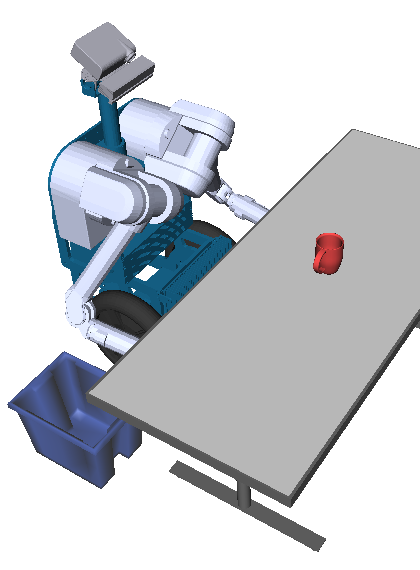
\includegraphics[width=1.4cm]{figs/herbbin/step0cropped.png}%
      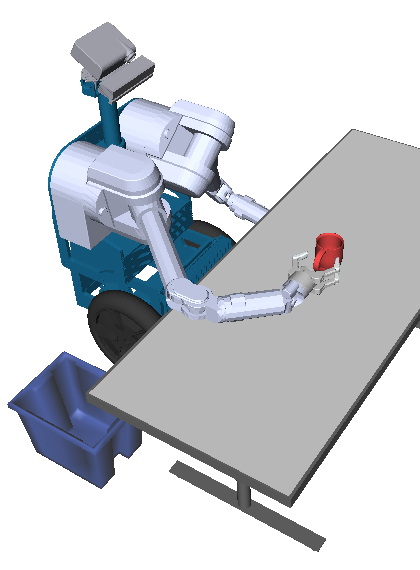
\includegraphics[width=1.4cm]{figs/herbbin/step01cropped.png}%
      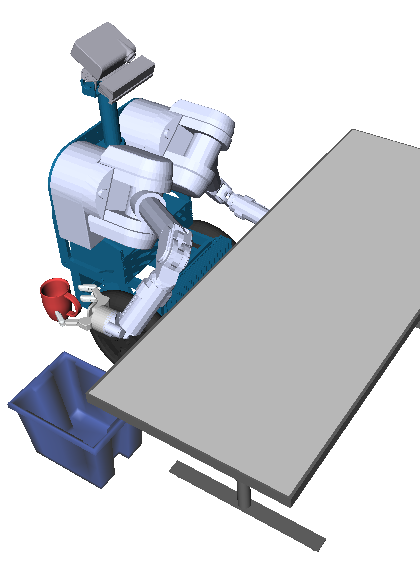
\includegraphics[width=1.4cm]{figs/herbbin/step12cropped.png}%
      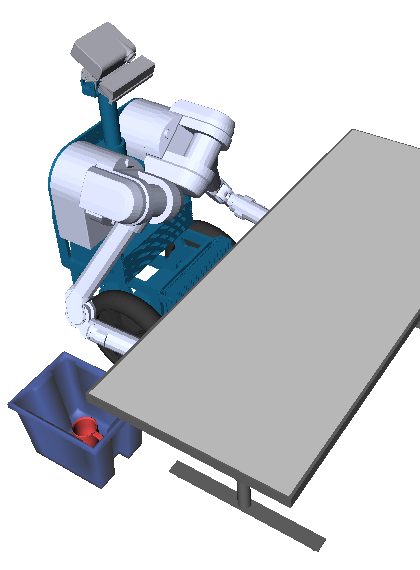
\includegraphics[width=1.4cm]{figs/herbbin/step2cropped.png}};

   \node[draw=black!40,rounded corners,inner sep=2pt,anchor=north] at (3.2,5.4)
      {\includegraphics[width=5.6cm]{build/workcell/configs}};

   \node[fill=blue!10,draw=blue!20,rounded corners,align=center,minimum width=5.3cm,minimum height=1.5cm,anchor=north] at (9.1,7.7)
   {$\arraycolsep=1.5pt \begin{array}{cl}
      x(\xi)\!: & \mbox{execution cost} \;(\mathcal{C}_{\ms{free}}) \\
      \hat{x}(\xi)\!: & \mbox{execution cost estimate} \\
      \grave{p}(\xi)\!: & \mbox{planning cost estimate}
   \end{array}$};

   \node[fill=black!2,draw=black!5,rounded corners,minimum width=5.3cm] at (9.1,3.7) {\begin{minipage}{5.0cm}
      Planning \& execution cost model:
      \[\arraycolsep=2pt \def\arraystretch{1.5} \begin{array}{clc}
         x(\xi)
            & = \left\{ \def\arraystretch{1.0} \begin{array}{cl}
               ||\xi|| & \mbox{if } \xi \in \mathcal{C}_{\ms{free}} \\
               \infty & \mbox{otherwise} \\
               \end{array} \right.
            & \mbox{(rad)} \\
         {\hat x}(\xi) & = ||\xi|| & \mbox{(rad)} \\
         {\grave p}(\xi) & = \alpha N_{\ms{cc}}(\xi) & \mbox{(sec)}
      \end{array}\]
      with $N_{cc}(\xi)$ the number of collision checks necessary
      to validate $\xi$,
      and $\alpha$ a fixed checking cost parameter.
   \end{minipage}};

   \end{tikzpicture}
\end{frame}

\begin{frame}
   \frametitle{LEMUR Single-Query Results}
   \begin{tikzpicture}[font=\small]
   \draw[step=1,black!15,very thin,opacity=\gridopacity] (0,0) grid (12,8);
   \tikzset{>=latex} % arrow heads

   \node[inner sep=0pt] (vizall-herbbin) at (3,6.5) {%
      \href{\tikzvidtarget{vizall-herbbin}}{%
      \includegraphics[width=5.8cm]{videos/vizall-herbbin.png}}};
   \tikzvidplayat{vizall-herbbin}{vizall-herbbin}{videos/vizall-herbbin.mp4}{}

   \node[inner sep=0pt] (vizall-workcell) at (9,6.5) {%
      \href{\tikzvidtarget{vizall-workcell}}{%
      \includegraphics[width=5.8cm]{videos/vizall-workcell.png}}};
   \tikzvidplayat{vizall-workcell}{vizall-workcell}{videos/vizall-workcell.mp4}{}
   
   \node[fill=black!2,draw=black!5,rounded corners,minimum width=5.3cm] at (6,3.5)
   {\begin{minipage}{9.0cm}
      Comparing utility across planners:
      \begin{itemize}
      \item 50 runs for each planner (randomized)
      \item 50 different roadmaps (random Halton offsets)
      \item LEMUR: sweep $\lambda$ tradeoff parameter
      \item Anytime algorithms: sweep optimization time budget
      \end{itemize}
   \end{minipage}};

   \end{tikzpicture}
\end{frame}
   
%\begin{frame}
%   \frametitle{Lazily Evaluated Marginal Utility Roadmaps}
%   \begin{tikzpicture}[font=\small]
%   \draw[step=1,black!15,very thin,opacity=\gridopacity] (0,0) grid (12,8);
%   \tikzset{>=latex} % arrow heads
%
%      \node[fill=blue!5,rounded corners,anchor=north,minimum width=9.5cm,minimum height=6.7cm] (alg) at (6,7.75) {};
%      \node[left=0.1cm of alg.north,anchor=north] {\begin{minipage}{9cm}
%         \begin{algorithmic}[1]
%         \Procedure {LEMUR}{$q_{\ms{start}}, q_{\ms{goal}}, x,
%            \mathcal{M}.\grave{p}, \mathcal{M}.\hat{x}, \lambda_p$}
%         \State $G \leftarrow$ graph with
%            $V = \{ q_{\ms{start}}, q_{\ms{goal}} \}$
%            and $E = \emptyset$
%         %\State $w_0 : E \rightarrow \mathbb{R}^{+}$ \Comment mutable edge weight function
%         \State $w_0(e) = \lambda_p \, \grave{p}(e) + (1\!-\!\lambda_p) \, \hat{x}(e) \quad \forall e \in G.E$
%         \For {iteration $i \in 1, 2, \dots$}
%            \State $\pi_i = \displaystyle\argmin_{\pi \in \Pi(G)} 
%               \mbox{len}\left(\pi, w\right)$
%               \Comment incremental search
%            \If {$\pi_i$ is {\bf null}}
%               \State $V_{\ms{new}}, E_{\ms{new}} \leftarrow$ new densified roadmap batch
%               \State $G.V \stackrel{\tiny +}\leftarrow V_{\ms{new}};
%                  \;\; G.E \stackrel{\tiny +}\leftarrow E_{\ms{new}}$
%               \State $w(e) \leftarrow \lambda_p \, \grave{p}_i(e) + (1\!-\!\lambda_p) \, \hat{x}_i(e)
%                  \; \forall \; e \in E_{\ms{new}}$
%               \State {\bf continue}
%            \EndIf
%            \If {$\pi_i$ is fully evaluated}
%               \State \Return $\pi_i$
%            \EndIf
%            \State $e_i \leftarrow$ select unevaluated edge from $\pi_i$
%            \State evaluate $e_i$
%            \State $\hat{x}(e_i) \leftarrow x(e_i); \;\; \grave{p}(e_i) \leftarrow 0$
%               \Comment e.g. evaluate fully
%            \State $w_i(e_i) \leftarrow
%               \lambda_p \, \grave{p}(e_i) + (1\!-\!\lambda_p) \, \hat{x}(e_i)$
%         \EndFor
%         \EndProcedure
%         \end{algorithmic}
%      \end{minipage}};
%
%
%   \end{tikzpicture}
%\end{frame}

\begin{frame}
   \frametitle{Maximizing Utility: HERB Table Clearing}
   \begin{tikzpicture}[font=\small]
      \tikzset{>=latex} % arrow heads
      \draw[step=1,black!15,very thin,opacity=\gridopacity] (0,0) grid (12,8);

      %\node[inner sep=0pt] (vidnode) at (9.5,6.5) {%
      %   \href{\tikzvidtarget{incbi-roadne}}{%
      %   \includegraphics[width=4cm]{videos/workcell-cropped.png}}};
      %\tikzvidplayat{incbi-roadne}{vidnode}{videos/workcell-cropped.mp4}{}

      \node at (6,4) {\includegraphics[width=11cm]{build/lemur-sq/herbbin0}};

      \node[fill=red,draw=black,inner sep=4pt] (rrtconnect) at (6.7,5.3) {};
      \node[anchor=west,right=0cm of rrtconnect.east] {\strut RRT Connect + Shortcutting};

      \node[fill=green,draw=black,inner sep=4pt] (bitstar) at (6.7,4.9) {};
      \node[anchor=west,right=0cm of bitstar.east] {\strut Batch Informed Trees (BIT*)};

      \node[fill=cyan,draw=black,inner sep=4pt] (lazyarastar) at (6.7,4.5) {};
      \node[anchor=west,right=0cm of lazyarastar.east] {\strut Lazy ARA*};

      \node[fill=black!80,draw=black,inner sep=4pt] (lemur) at (6.7,4.1) {};
      \node[anchor=west,right=0cm of lemur.east] {\strut LEMUR};

      \node[draw=black!40,rounded corners,inner sep=2pt,anchor=north,fill=white] at ( 9,7.9) {
         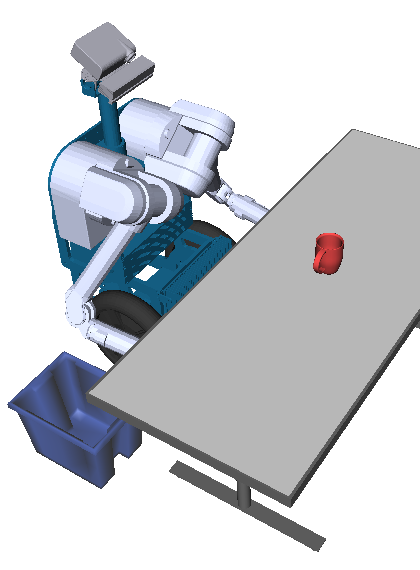
\includegraphics[width=1.4cm]{figs/herbbin/step0cropped.png}
         \;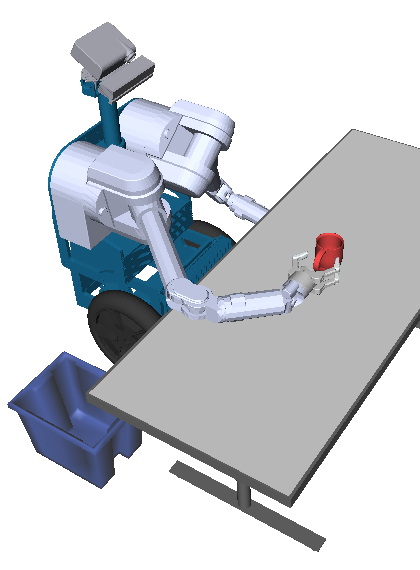
\includegraphics[width=1.4cm]{figs/herbbin/step01cropped.png}};
      
   \end{tikzpicture}
\end{frame}

\begin{frame}
   \frametitle{Maximizing Utility: IRB4400 Industrial Workcell}
   \begin{tikzpicture}[font=\small]
      \tikzset{>=latex} % arrow heads
      \draw[step=1,black!15,very thin,opacity=\gridopacity] (0,0) grid (12,8);

      %\node[inner sep=0pt] (vidnode) at (9.5,6.5) {%
      %   \href{\tikzvidtarget{incbi-roadne}}{%
      %   \includegraphics[width=4cm]{videos/workcell-cropped.png}}};
      %\tikzvidplayat{incbi-roadne}{vidnode}{videos/workcell-cropped.mp4}{}

      \node at (6,4) {\includegraphics[width=11cm]{build/lemur-sq/workcellfg}};

      \node[fill=red,draw=black,inner sep=4pt] (rrtconnect) at (6.7,5.3) {};
      \node[anchor=west,right=0cm of rrtconnect.east] {\strut RRT Connect + Shortcutting};

      \node[fill=green,draw=black,inner sep=4pt] (bitstar) at (6.7,4.9) {};
      \node[anchor=west,right=0cm of bitstar.east] {\strut Batch Informed Trees (BIT*)};

      \node[fill=cyan,draw=black,inner sep=4pt] (lazyarastar) at (6.7,4.5) {};
      \node[anchor=west,right=0cm of lazyarastar.east] {\strut Lazy ARA*};

      \node[fill=black!80,draw=black,inner sep=4pt] (lemur) at (6.7,4.1) {};
      \node[anchor=west,right=0cm of lemur.east] {\strut LEMUR};

      \node[draw=black!40,rounded corners,inner sep=2pt,anchor=north,fill=white] at ( 9,7.9) {
         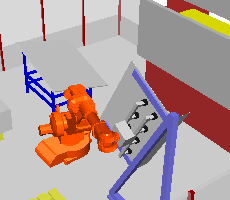
\includegraphics[width=2.0cm]{figs/workcell/cropped-config-f.png}
         \;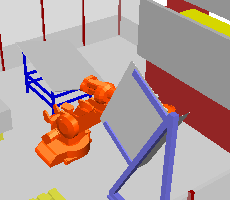
\includegraphics[width=2.0cm]{figs/workcell/cropped-config-g.png}};
      
   \end{tikzpicture}
\end{frame}

%\begin{frame}
%   \frametitle{Maximizing Utility: Workcell Experiments}
%   \begin{tikzpicture}[font=\small]
%      \tikzset{>=latex} % arrow heads
%      \draw[step=1,black!15,very thin,opacity=\gridopacity] (0,0) grid (12,8);
%
%      \node at ( 3.75,6.4) {
%         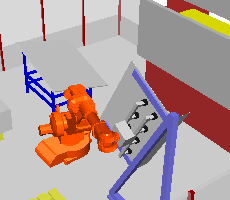
\includegraphics[width=2.7cm]{figs/workcell/cropped-config-f.png}
%         \;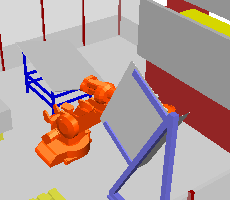
\includegraphics[width=2.7cm]{figs/workcell/cropped-config-g.png}};
%
%      \node[inner sep=0pt] (vidnode) at (9.5,6.5) {%
%         \href{\tikzvidtarget{workcell-cropped}}{%
%         \includegraphics[width=4cm]{videos/workcell-cropped.png}}};
%      \tikzvidplayat{workcell-cropped}{vidnode}{videos/workcell-cropped.mp4}{}
%
%      \node at (3.5,2.5) {\includegraphics[width=7cm]{build/lemur-sq/workcellfg}};
%      
%   \end{tikzpicture}
%\end{frame}

%\begin{frame}
%   \frametitle{Maximizing Utility: Workcell Experiments (multistep)}
%   \begin{tikzpicture}[font=\small]
%      \tikzset{>=latex} % arrow heads
%      \draw[step=1,black!15,very thin,opacity=\gridopacity] (0,0) grid (12,8);
%
%      \node at ( 3.75,6.4) {
%         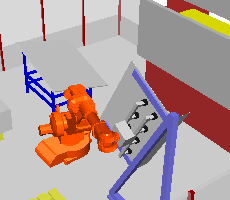
\includegraphics[width=2.7cm]{figs/workcell/cropped-config-f.png}
%         \;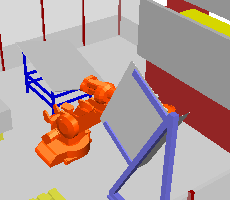
\includegraphics[width=2.7cm]{figs/workcell/cropped-config-g.png}};
%
%      \node[inner sep=0pt] (vidnode) at (9.5,6.5) {%
%         \href{\tikzvidtarget{workcell-cropped}}{%
%         \includegraphics[width=4cm]{videos/workcell-cropped.png}}};
%      \tikzvidplayat{workcell-cropped}{vidnode}{videos/workcell-cropped.mp4}{}
%
%      \node at (2.5,2.5) {\includegraphics[height=4cm]{build/multistep-prescribed/herbbinnom-g1ll-lemuronly}};
%
%      \node at (9.5,2.5) {\includegraphics[height=4cm]{build/multistep-prescribed/workcell-g1ll-lemuronly}};
%      
%   \end{tikzpicture}
%\end{frame}
